\documentclass{article}
\usepackage{listings}
\usepackage[utf8]{inputenc}
\usepackage{graphicx}

\graphicspath{{../results/}}

\lstset{
	basicstyle=\footnotesize,
	numbers=left,
	tabsize=3,
	title=\lstname,
	breaklines=true
}

\addtolength{\oddsidemargin}{-.875in}
\addtolength{\evensidemargin}{-.875in}
\addtolength{\textwidth}{1.75in}

\addtolength{\topmargin}{-.875in}
\addtolength{\textheight}{1.75in}

\title{Neuronale Netze - Übung 8}
\author{Tobias Hahn\\ 3073375}	
	
\begin{document}
\maketitle
\newpage
\section{Neuronales Netz}
\subsection{Implementierung}
Meine Implementierung hat wohl einen Fehler, ich bin aber leider nicht dahintergekommen wo. Die Deltas werden wie gewohnt berechnet, nur werden, wie gefordert, am Ende für das Update nicht die Inputs als fix betrachtet sondern die Gewichte, um so den Gradienten für die Inputs zu bekommen. Das Bild ändert sich jedoch nicht viel, und vor allem nicht zwischen den Durchgängen. Woran das liegt kann ich nicht sagen. Ich habe versucht für die Berechnung der Delta auch die Signale statt der Gewichte zu benutzen, dies führte jedoch zum selben Ergebnis.

\subsection{Code}
Der Code des Netzes ist hier:
\paragraph{}
\lstinputlisting[language=Python]{../code/NeuralNet.py}
\lstinputlisting[language=Python]{../code/train.py}

\subsection{Ergebnisse}
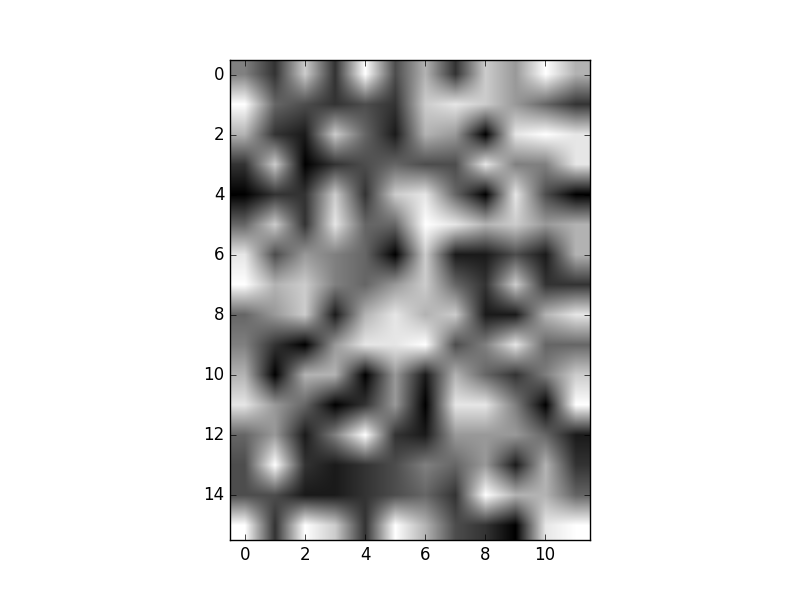
\includegraphics[width=\textwidth]{dream}
\end{document}
